% Shared panel dimensions, baselines, typography and colours with the other
% introduction figures. The scenes are illustrative, not measured results.
\begin{tikzpicture}[
  imgnode/.style={inner sep=0pt, draw=black!35, line width=1.0pt},
  titletext/.style={font=\bfseries},
  captiontext/.style={font=\small\itshape, align=center, text width=6.6cm},
  desctext/.style={font=\small, align=center, text width=6.6cm},
  decisiontext/.style={font=\small, align=center, text width=6.6cm,
    text=steelblue31119180!70!black},
]
\node[imgnode] (chess) {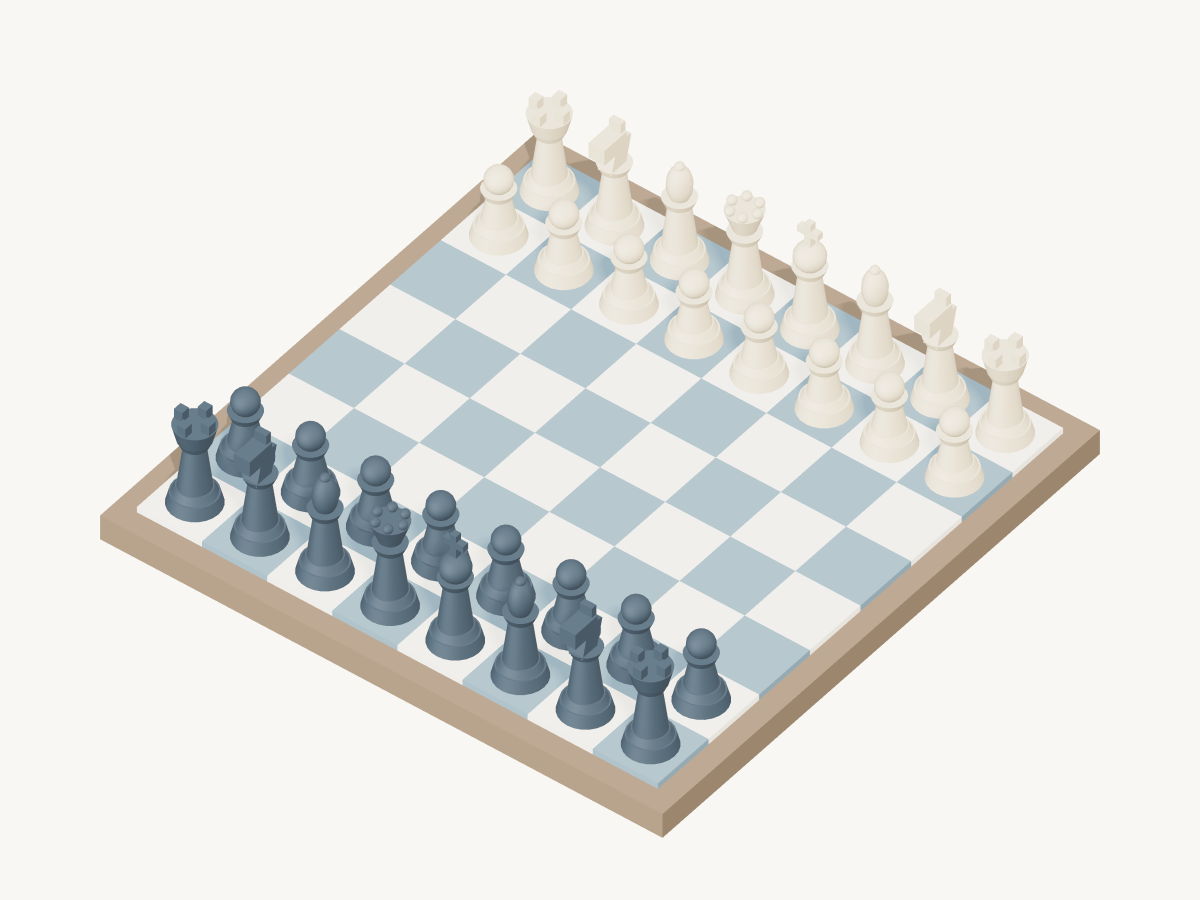
\includegraphics[width=6.6cm]{img/main/three/renders/moravec_chess.png}};
\node[imgnode, right=2.0cm of chess] (crowd) {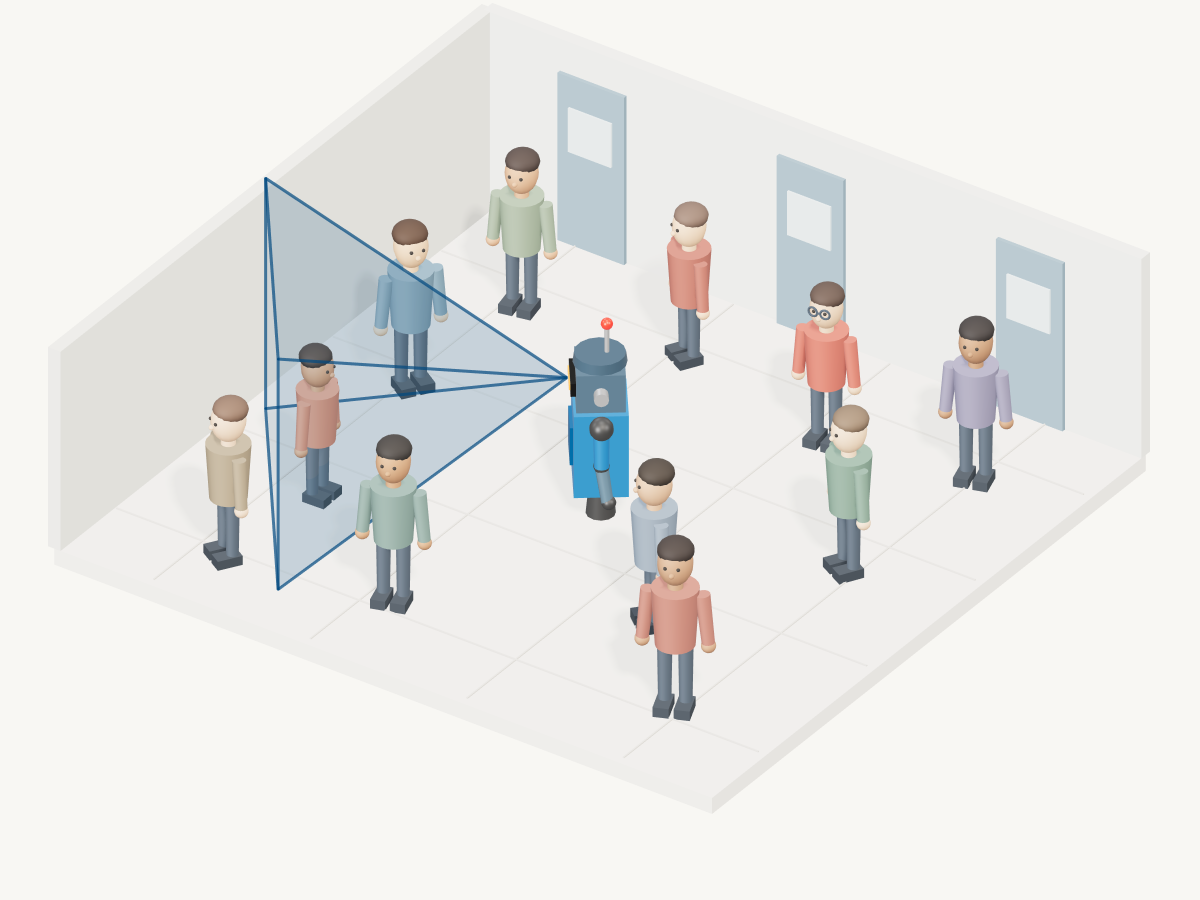
\includegraphics[width=6.6cm]{img/main/three/renders/moravec_crowd.png}};
\node[titletext] (lefttitle) at ($(chess.north)+(0,1.0)$) {Formal intellectual task};
\node[titletext, anchor=base] at (crowd.center |- lefttitle.base) {Everyday visual task};
\node[captiontext] (leftsub) at ($(chess.north)+(0,0.43)$) {choose a move in chess};
\node[captiontext, anchor=base] at (crowd.center |- leftsub.base) {find a familiar person};
% Reference portrait shows the person to find without marking their location.
\node[imgnode, anchor=north west] (portrait) at ($(crowd.north west)+(0.14,-0.14)$)
  {
\includegraphics[width=1.05cm]{img/main/three/renders/moravec_portrait.png}};
\node[font=\scriptsize, fill=white, inner sep=1pt, anchor=north,
  text width=1.05cm, align=center, text=black!80] at (portrait.south) {find this\\person};
\node[desctext, anchor=north] at ($(chess.south)+(0,-0.25)$)
  {Explicit rules and objective\\Relevant game state available};
\node[desctext, anchor=north] at ($(crowd.south)+(0,-0.25)$)
  {Occlusion and incomplete views\\Limited time to gather evidence};
\node[decisiontext, anchor=north] at ($(chess.south)+(0,-1.25)$)
  {Evaluate possible moves\\within a defined problem};
\node[decisiontext, anchor=north] at ($(crowd.south)+(0,-1.25)$)
  {Choose where to look, recognise the person,\\and decide when enough has been seen};
\draw[black!45, line width=0.4pt]
  ($(chess.north east)+(1.0,1.25)$) -- ($(chess.south east)+(1.0,-2.1)$);
\end{tikzpicture}
